\documentclass[../../time_series_notes.tex]{subfiles}
\begin{document}
%%%%%%%%%%%%%%%%%%%%%%%%%%%%%%%%%%%%%%%%%%%%%%%%%%%%%%%%%%%%
\section{Exponential Smoothing with Trend}
\subsection{Holt's Linear Trend Method}
Also known as \textbf{Double Exponential Smoothing}, This method extends the simple smoothing method with a trend component. We will use $x$ and $l$ interchangeably.
\begin{align*}
    x_{t+h|t} &= l_{t} + hb_{t}\\
    l_{t} &= \alpha x_{t} + (1-\alpha)x_{t|t-1}\\
    &= \alpha x_{t} + (1-\alpha)(l_{t-1} + b_{t-1})\\
    b_{t} &= \beta(l_{t} - l_{t-1}) + (1-\beta)b_{t-1}
\end{align*}

where $l$ is the level and $b$ is the trend. The level equation is same as simple exponential smoothing, weighted sum of the series value at last time step and the forecasted value at the last time step ($l_{t-1} + 1 \times b_{t-1}$). The new component of trend is a weighted sum of trend estimate at last time step and the trend adjusted by taking the difference in levels.\newline

Both $\alpha, \beta \in [0,1]$. With the introduction of trend in the model, the forecast is no longer flat but linear in $h$. Figure \ref{fig:ses_trend_1} shows an example of how the levels and trends look for this method. The level is simliar to the series but the trend shows how much the values change at each time step.

\begin{figure}[h]
    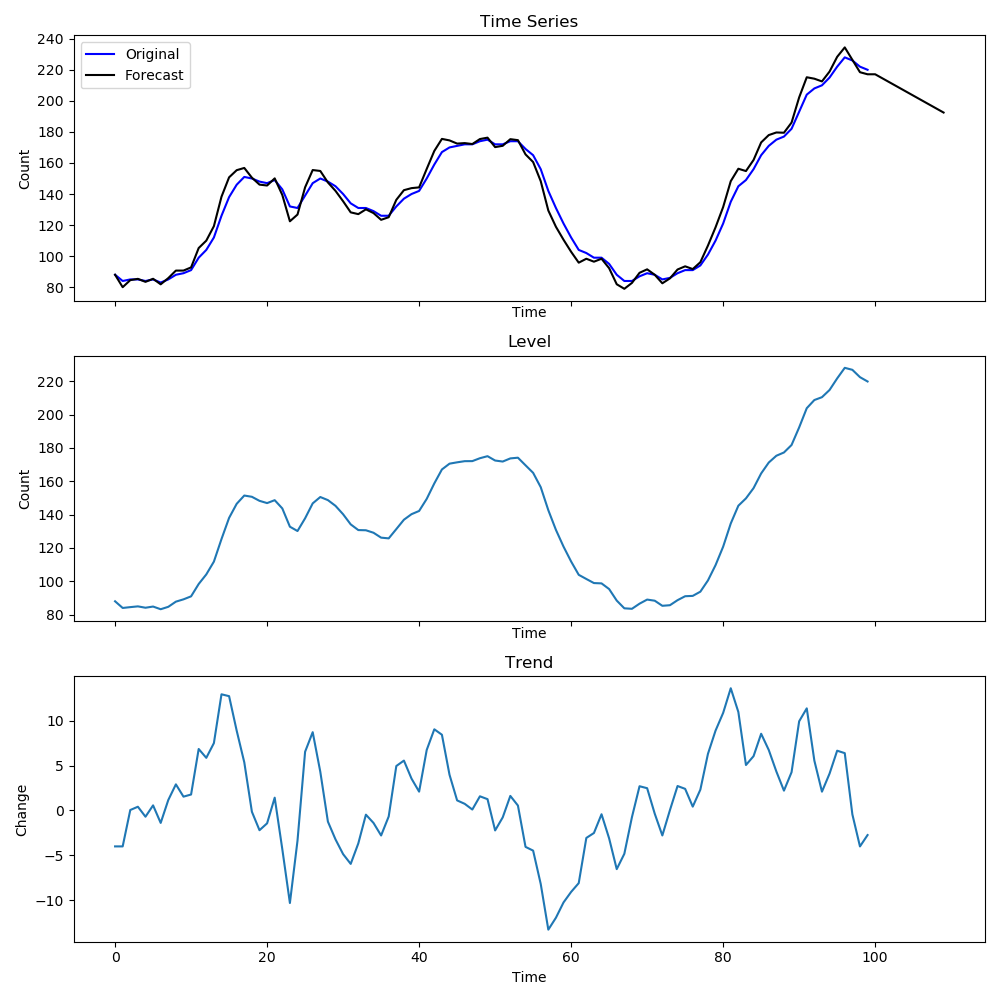
\includegraphics[scale=0.6]{ses_trend_1}
    \centering
    \caption {Top figure shows the original and forecasted series for $alpha=0.9$ and $\beta=0.9$. The forecast for future data is downwards linear due to the local trend there. Middle and bottom figures show the level and trend series that were calculated while running the algorithm. Figures plot using ses\_trend.py}
    \label{fig:ses_trend_1} %\ref{fig:ses_trend_1}
\end{figure}


\subsection{Damped Trend Method}
This method extends the above method to introduce variation in the trend. Since we do not expect the trend to remain the same, introducing some non-linearity can help reduce forecast errors. We introduce a dampening parameter $0 < \phi < 1$ into the previous method
\begin{align*}
    x_{t+h|t} &= l_{t} + (\phi + \phi^{2} + \cdots + \phi^{h})b_{t}\\
    l_{t} &= \alpha x_{t} + (1-\alpha)x_{t|t-1}\\
    &= \alpha x_{t} + (1-\alpha)(l_{t-1} + \phi b_{t-1})\\
    b_{t} &= \beta(l_{t} - l_{t-1}) + (1-\beta)\phi b_{t-1}    
\end{align*}

Notice that as $\phi \to \infty$, $x_{t+h|t} \to l_{t} + \phi b_{t}/(1-\phi)$ which means that for short term forecasts, the dampening will introduce variation, but long term forecasts will be near constant.  In practice, $\phi \in [0.8, 0.98]$ as dampening has a strong effect on short term values, and $\phi$ close to 1 will reduce to a non-damped model.
\end{document}